%%%%%%%%%%%%%%%%%%%%%%%%%%%%%%%%%%%%%%%%%%%%%%%%%%%%%%%%%%%%%%%%%%%%%%%%%%%%%%%%%%%
%%                 PŘÍLOHA - UŽIVATELSKÁ PŘÍRUČKA                                %%
%%%%%%%%%%%%%%%%%%%%%%%%%%%%%%%%%%%%%%%%%%%%%%%%%%%%%%%%%%%%%%%%%%%%%%%%%%%%%%%%%%%
\chapter{Srovnání polygonizace v ArcGIS a QGIS}
\label{chap:srovnani}
Srovnání bylo provedeno na testovacích datech, které poskytl \textit{Ing. Jan Růžička, Ph.D.}. Jelikož nemohla být poskytnuta reálná data, jedná se o uměle vygenerované linie, které jsou dle slov doktora Růžičky obdobného charakteru a velikosti, jako linie pro vytvoření pátracích sektorů v projektu Pátrač. Data obsahují celkem 10000 linií. Tato data byla dále testována ve zmenšené formě a to s 1000 a 100 liniemi.

\section{Parametry počítače}
\begin{itemize}
\item \textbf{Operační systém:} Windows 10 Enterprice LTSC
\item \textbf{Výrobce:} HP
\item \textbf{Model:} Z240
\item \textbf{Procesor:} Intel(R) Core(TM) i7-7700 CPU @3.60GHz 3.60GHz, 64bit
\item \textbf{RAM:} 32,0 GB
\end{itemize}

\section{Výsledky a porovnání}
Pro každý dataset byla provedena 5x polygonizace v jednotlivých softwarech a výsledný čas byl spočítán jako aritmetický průměr. Na datech co byla použita pro test nám nevzniká nějaký zásadní rozdíl se zvětšujícím se datasetem a oba nástroje se chovají velmi podobně. Výsledky jsou uvedeny v tabulce \ref{tab:srovnani}.

\begin{table}
\begin{tabular}{ |p{1.4cm}||p{1.2cm}|p{1.2cm}|p{1.2cm}|p{1.2cm}|p{1.2cm}|p{2.2cm}|  }
\hline
\multicolumn{7}{|c|}{ArcGIS} \\
\hline
linií			&1. $[s]$	&2. $[s]$	&3. $[s]$	&4. $[s]$	&5. $[s]$	&průměr\\
\hline
$100$			&0,41		&0,40		&0,40		&0,40		&0,40		&\textbf{0,40s}\\			
$1000$			&13,56		&13,57		&13,58		&13,57		&13,55		&\textbf{13,57s}\\
$10000$			&768		&792		&769		&774		&768		&\textbf{12min 54s}\\
\hline
\hline
\multicolumn{7}{|c|}{QGIS} \\
\hline
linií			&1. $[s]$	&2. $[s]$	&3. $[s]$	&4. $[s]$	&5. $[s]$	&průměr\\
\hline
$100$			&0,16		&0,06		&0,07		&0,06		&0,06		&\textbf{0,08s}\\			
$1000$			&10,02		&9,95		&9,98		&9,96		&9,97		&\textbf{9,98s}\\
$10000$			&748,00		&768,21		&751,74		&753,92		&757,29		&\textbf{12min 36s}\\
\hline
\end{tabular}
\caption{Srovnání časů výpočtu polygonizace v ArcGIS a QGIS.}
\label{tab:pr_srovnani_casu}
\label{tab:srovnani}
\end{table}

\begin{figure}[h]
  \centering
  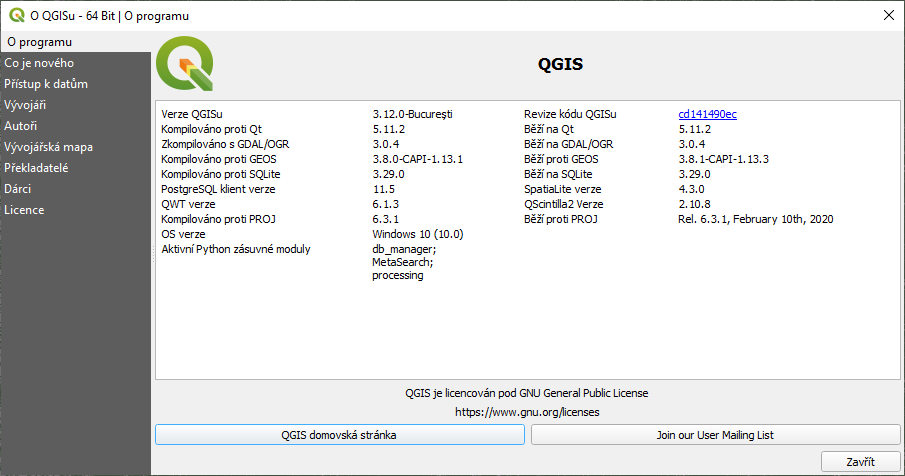
\includegraphics[width=12cm]{./pictures/prilohy/qgis_about.png}
  \caption{Verze QGIS.}
  \label{fig:qgis_about}
\end{figure}

\begin{figure}[h]
  \centering
  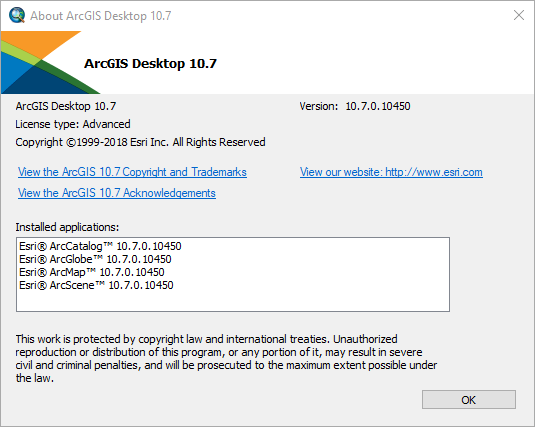
\includegraphics[width=12cm]{./pictures/prilohy/arcgis_about.png}
  \caption{Verze ArcGIS.}
  \label{fig:arcgis_about}
\end{figure}






\chapter{Elektornické přílohy}
\label{user-guide}

\section{CD disk}

\pagenumbering{Roman}
\label{app:cd}
    
    \begin{description}
        \item[\tt BP-DistortionRemover.pdf] ~ \\ text bakalářské práce ve formátu *.pdf,
    	
        
        \item[\tt DistortionRemover/] ~ \\ adresář s programem,
        \begin{description}
        		
        		\item[\tt DistortionRemover.exe] ~ \\ Spustitelný soubor aplikace,
        		
        		\item[\tt License.txt] ~ \\ textový soubor s popisem licence,
        		
            	\item[\tt Source/] ~ \\ adresář obsahující zdrojové kódy,
            	\begin{description}
            			\item[\tt DistortionRemover.pro] ~ \\ projektový soubor,
            			\item[\tt main.cpp] ~ \\ zdrojový kód funkce main,
            			\item[\tt distortionremover.h] ~ \\ hlavičkový soubor distortionremover,
            			\item[\tt distortionremover.cpp] ~ \\ zdrojový soubor distortionremover obsahující funkce pro chod programu,
            			\item[\tt ui\_distortionremover.h] ~ \\ hlavičkový soubor grafického rozhraní,
            			\item[\tt distortionremover.ui] ~ \\ soubor obsahující grafické prostředí v XML,
            			\item[\tt picturetransformation.h] ~ \\ hlavičkový soubor picturetransformation,
            			\item[\tt picturetransformation.cpp] ~ \\ zdrojový soubor picturetransformation obsahující výpočetní funkce,
            			\item[\tt resource.qrc] ~ \\ soubor pro uložení binárních souborů do aplikace který obsahuje ikonu,
            			\item[\tt DR.ico] ~ \\ ikona programu.

            	\end{description}
        \end{description}
    \end{description}

